\scanpage{16}
\mspage{\unsure{3|5})}
\textcircled{3} Let
\deleted{$X\supset Y$, $X$ \unsure{equipped with subspaces}}
\inserted{$T$ be an absolute \deleted{tubular} conical neighborhood of $Y$.}
% P03: the epsilon-like lowered group is overworked; no independent strike establishes its cancellation state.
\unsure{Let|Let} $\unsure{T'_\varepsilon|T'\deleted{_\varepsilon}}\subset T$.
We say that $T'$ is a \uline{conical subspace} in $T$ if we have
\[
(12)\qquad\left\{\begin{array}{ll}
a)&T'\text{ stable under homotheties }\lambda\in\mathbf{I}\qquad
\deleted{\unsure{\lambda T'\subset T'}}\\
% P04: the initial P has a small raised/retraced remnant, without a recoverable earlier token.
b)&\text{\unsure{For} this action, }T'\text{ is a neighborhood}
\end{array}\right.
\]
\deleted{tubular} conical of $Y$.
\uline{NB} We shall necessarily have $\unsure{\dot T'}=T'\cap\dot T$,
$T'_\lambda=T'\cap T_\lambda$ ;
\deleted{If $(T_i)_{i\in I}$ is a family\unsure{,}}
\inserted{the datum of $T'$ is equivalent to}
that of a closed subspace $\dot T'$ of $\dot T$
and of a subspace $\unsure{T'|Y'}$ of $Y$, such that $Y'\supset0.\dot T'$, and,
we have
\[
% P08: separate unrecoverable raised mark above the double-stem I; no established accent meaning or cancellation state.
T'=\operatorname{Im}(\overset{\unsure{}}{\mathbb{I}}\times
\dot T'\unsure{\lambda|\deleted{\lambda}|\ell|\}}
\unsure{\mathrel{\relbar\joinrel\relbar}|\longrightarrow}T)\cup Y'.
\]
\margin{We say that $T'$ is \uline{strictly} conical
if $T'\cap Y=0.\dot T'$
--- these $T'$ thus correspond to the closed subsets
$\dot T'$ of $\dot T$.}

We shall say that a conical structure on
a $T\supset Y$ is \uline{compatible} with \inserted{closed} subspaces
$T_i$ of $T$ $(i\in I)$ if the latter
are conical for this structure.

Let $T$ be a conical neighborhood of $Y\subset X$
in $X$, let $X'$ be a closed \unsure{s}ubset of $X$. We
% P11/P12: the apparent mark above the end of compatible belongs to the hooked descender of fermée.
say that $T$ is \uline{compatible} with $X'$ if
$X'\cap T$ is conical in $T$. We say that it
is \uline{strictly compatible}$^{*}$ with $T$, if
$T$ is a strict conical neighborhood, and if there exists
a cylindrical neighborhood of $\dot T$ in
$X^*=X\setminus\mathring T$, compatible with
$X'{}^{\unsure{*|\mathrm r}}=X'\cap X^*$,
or what amounts to the same, if there exists a
neighborhood $E$ of $\dot T$ in $X^*$, and an isomorphism
\margin{\deleted{\unsure{Define the notion for $X'$|say \illegible{1} compatible with $X'$}}}
\margin{$^{*}$ \deleted{\uline{\unsure{also say|transverse}} \uline{\unsure{strict}}}}
\margin{\unsure{probably} modify the definition of
\unsure{strict|strict} conical neighborhoods\ldots}
% P18: one unheaded separator/leader beside the lower marginal note, leaning slightly right down the original page.
\margin{\figure{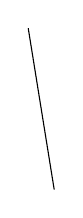
\begin{tikzpicture}[x=1cm,y=1cm]
\draw (0,0)--(0.33,-2.05);
\end{tikzpicture}}}
\margin{15}
